
\documentclass{ijcaArticle}
\setcounter{page}{1}
\ijcaVolume{VV}
\ijcaNumber{N}
\ijcaYear{YYYY}
\ijcaMonth{Month}

\ijcaVolume{*}
\ijcaNumber{*}
\ijcaYear{2012}
\ijcaMonth{--------}
\begin{document}

\title{High Speed Data Communication using LiFi providing Security} % title

\author{ 
   \large Nadeem Patil \\[-3pt]
   \normalsize JSPM's Imperial College of Engineering and Research  \\[-3pt]
    \normalsize Wagholi, Pune \\[-3pt]
    \normalsize	nadeemp77@live.in \\[-3pt]
  \and
   \large Abhijit Jirole \\[-3pt]
   \normalsize JSPM's Imperial College of Engineering and Research  \\[-3pt]
    \normalsize Wagholi,Pune \\[-3pt]
    \normalsize	abhijirole123@gmail.com \\[-3pt]
\and
   \large Hemant Badhe \\[-3pt]
   \normalsize JSPM's Imperial College of Engineering and Research  \\[-3pt]
    \normalsize Wagholi, Pune \\[-3pt]
    \normalsize	hemantbadhe1305@gmail.com \\[-3pt]
    \and
   \large Pramodini Akhade \\[-3pt]
   \normalsize JSPM's Imperial College of Engineering and Research  \\[-3pt]
    \normalsize Wagholi, Pune \\[-3pt]
    \normalsize	akhadepramu@gmail.com \\[-3pt]
}

\terms{Visible Light Communication(VLC), High Speed Data Transmission, Data Transmission Security }
\keywords{Arduino Microcontroller, Light Emitting Diode(LED), Photo diode, Wireless communication}

\maketitle



\begin{abstract} 
Data communication or transmission has become the most demanding need
for the most of the computer users. Security is another more important concern when it
comes to establishing communication between systems through the network. LiFi technology
is focused on fulfilling these demands. LiFi basically uses Visible Light Communication(
VLC) to establish connection and transmit data. The transmission rate of
visible light is faster than all other available today transmission medias such as WiFi,
ethernet, infrared, etc. Visible Light Communication has many features such as High
speed, no radiation, easy to use, easy installation and management, etc. However exiting
LiFi misses out some things such as two way communication, security. So in order to
achieve the high speed of LiFi technology and provide transmission security, the proposed
system provides the necessary information which can make the system usable.
\end{abstract}

\section{Introduction}

Data communication or the transmission among various systems is the most commonly used feature
of the computer systems. There are various data transmission methods such as wired communication,
wireless communication. Ethernet, WiFi, Bluetooth are the widely used data transmission protocols.
With the increasing number of computer users, the data storage capacities and data requirements are
increasing tremendously. The existing systems are facing various issues such as traffic overloading
, data bottleneck, bandwidth overloading, etc. To overcome these issues, we require even the higher
bandwidth than existing systems. LiFi has the capability to fulfil this demand so, bringing the LiFi
technology in use can solve many issues. Additionally, security needs to be maintained for data integrity
and reliability. The basic idea of the project is to reduce bandwidth overloading, network traffic,
communication restrictions in sensitive areas, etc. and provide secure, reliable and easy to use system
for users.



\section{Existing System}
\label{sec:documentclass}
The communication among various devices nowadays is done through various wired and wireless communication protocols. The LiFi system is currently least used due to some of its limitations, existing LiFi system is limited to one  way communication. It does not provide any kind of security at the moment. The basic idea behind this project is to eliminate limitations of the existing LiFi System. The existing system currently acts as a broadcasting service only which does not have any method to take user input.
\section{Proposed System}

The proposed system uses Arduino Uno R3-328 and MSP 430 G2 micro controllers. These micro
controllers are capable of connecting to personal computers and can be programmed through programming
languages. The primary goal of the system is to provide high data transmission rate and
should also provide the data security. With the increased data traffic, the speed expectations
also increase. LiFi has the ability to fulfil this expectation through its high bandwidth capacity.
Adding security to this feature involves bringing forward the encryption method. A data encryption method is used to provide the proper data security. This makes sure that the data transmission in progress is not eavesdropped, stolen or tampered. Along with this users are provided with uninterrupted high bandwidth data transmission which is not limited to one way communication. Providing two way communication with proper synchronisation is the primary focus of this system.

\section{Arduino Microcontroller}
\begin{figure}[h]
\centering
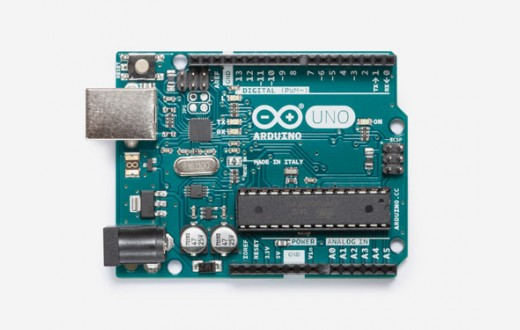
\includegraphics[width=2in]{Arduino.jpg}
\caption{Arduino Uno R3-328}
\label{fig:Arduino Uno}
\end{figure}

Arduino is a microcontroller which is open-source electronics platform. It is based on easy-to-use hardware and software.
Arduino is capable of reading input and turning it to some output. It is very much useful in most of the practical applications which require input through some sensing devices or manual user input. Arduino used in our system will be attached to LED devices and Photo diodes for performing data transmission. It can easily be programmed through the programming languages. The languages supported by Arduino are Object Oriented hence are easy to understand and program.


\section{Light Emitting Diode(LED)}
\label{sec:additional_faci}

\begin{figure}[h]
\centering
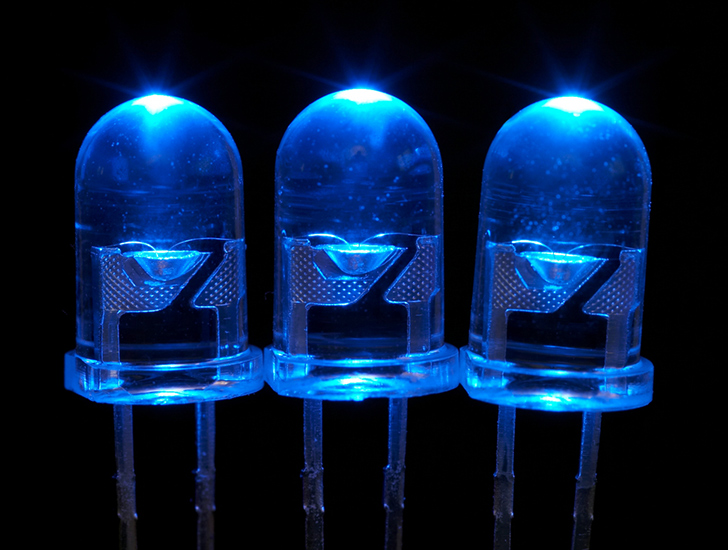
\includegraphics[width=2in]{LED.jpg}
\caption{Light Emitting Diode}
\label{fig:Light Emitting Diode}
\end{figure}
Light Emitting Diode is a device which is capable of producing light. This device can be controlled by the Arduino microcontroller. This device can manage high frequency turning ON or  OFF of itself. The ON state of LED represents binary 1 and OFF represents binary 0. This device can withstand in many environmental states such as high temperature, high magnetic field, underwater, etc.

\section{Photo Diode}
\label{sec:additional_faci}

\begin{figure}[h]
\centering
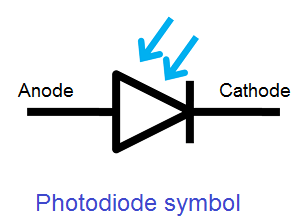
\includegraphics[width=2in]{PhotoDiode.png}
\caption{PhotoDiode}
\label{fig:Photo Diode}
\end{figure}
A photodiode is a semiconductor device that converts light into an electrical current. This device is able to absorb the falling light or the photons and convert it to electrical energy. A photodiode can also consist of optical filter. This device acts as a receiving device in our proposed system. A photodiode is connected with Arduino and Arduino passes it to the receiving computer. Photodiode is  useful device as it is cheaper and easy to use. Installation of the photodiode is pretty easy  as it can be directly connected to the microcontroller and does not require any additional device.

\section{Wireless Communication}
\label{sec:additional_faci}
The term wireless communication refers to the transmission of data among various devices without having connected by any physical medium. The existing wireless communication protocols are WiFi, Bluetooth, WiMax, etc. These protocols are not using any physical medium for interaction also these are not visible for human eyes. Visible Light communication is also a Wireless communication method but human eye can detect the light used for communication. Wireless communication methods are preferred as these are easy to install and usually are less costly than wired protocols.

\section{Comparision and Analysis}
\label{sec:additional_faci}

\begin{figure}[h]
\centering
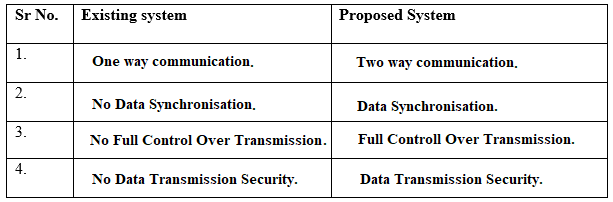
\includegraphics[width=3.8in]{comp.png}
\end{figure}

\section{ACKNOWLEDGEMENT }
We would like to take this opportunity to thank  Prof.A. Bharate for giving us all the help and guidance we needed. We are really grateful for her kind support. Her valuable suggestions were very helpful.
We are also grateful towards Dr. S. R. Todmal, for his indispensable support and suggestions for time to time.

\section{References}

\textbf{[1]} Zashi P. Chaudhari, Satish R. Devane, "High sensitivity universal LiFi receiver for enhanced data communication", IEEE, 2016.\\
\\
\textbf{[2]} Monica Leba, Simona Riurean, Andreea Lonica, "LiFi The path to a New Way of Communication", IEEE, 2017. \\
\\
\textbf{[3]} R. Mahendran, "Integrated LiFi (Light Fidelity) for smart communication through illumi-
nation",IEEE,  2016.\\
\\
\textbf{[4]} Harald Hass, "LiFi: Conceptions, misconceptions and opportunities",IEEE,  2016.\\
\\
\textbf{[5]} Pradeep Kumar, "Future internet and Internet of things", IEEE, 2017.\\
\\
\textbf{[6]} Kun Chen Hu, "Prototyping and measurements for a LiFi system", IEEE, 2016.\\
\\
\textbf{[7]} Dahmani Mohammed, "Digital data transmission via visible light communication(VLC): Applica-
tion vehicle to vehicle communication", IEEE, 2016.\\
\\
\textbf{[8]} Wasiu O. Popoola, "Impact of VLC on Light Immission Quality of White LEDs", IEEE, 2016.\\
\\
\textbf{[9]} Wasiu O.Popoola, "On visible light communication and quality of light emitted from illumi-
nation LEDs", IEEE, 2016.\\






\end{document}